\section{MOS Operationsverstärker}
'Operationsverstärker' ist ein \textbf{Sammelbegriff} für Differenzverstärker mit sehr grosser Verstärkung.

\smallskip

Der \textbf{ideale} Operationsverstärker erfüllt zwei Bedingungen:
\begin{itemize}
    \item Es fliesst kein Strom in die Eingänge
    \item Die Spannungsdifferenz zwischen den Eingängen ist null
\end{itemize}

\medskip

Man unterscheidet dabei zwischen \textbf{zwei Arten} von Operationsverstärkern:
\begin{description}
    \item[OTA:] Der Transimpedanz-Operationsverstärker hat eine Spannung am Eingang und liefert am Ausgang einen Strom
    \item[OpAmp:] Der OpAmp verstärkt die Eingangsspannung zu einer Ausgangsspannung 
\end{description}

\begin{ctabular}{|c|c||c|c|}
    \hline
    \multicolumn{2}{|c||}{\textbf{OTA}}                 & \multicolumn{2}{c|}{\textbf{OpAmp}}           \\
    \hline
    $Z_{\rm in} \to \infty$ & $Z_{\rm out} \to \infty$  & $Z_{\rm in} \to \infty$ & $Z_{\rm out} \to 0$ \\
    \hline
\end{ctabular}

\vspace{-0.2cm}


\subsection{Struktur}
\label{Struktur}

\begin{center}
    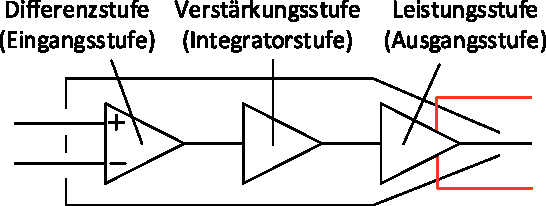
\includegraphics[width=0.65\columnwidth]{images/09_OpAmp_struktur.pdf}
\end{center}

\begin{outline}
    \1 \textbf{Differenzstufe}
        \2 Bildet die Differenz zwischen $V+$ und $V-$ und verstärkt diese
    \1 \textbf{Verstärkerstufe}
        \2 Erhöht die Verstärkung und bestimmt meist die Bandbreite
    \1 \textbf{Leistungsstufe}
        \2 Wandelt die hohe Impedanz in eine kleine Ausgangsimpedanz
            \textrightarrow\ \textbf{fehlt beim OTA}
\end{outline}


% \subsubsection{Differenzstufe}
% Bildet die Differenz zwischen $V+$ und $V-$ und verstärkt Differenzstufe

% \subsubsection{Verstärkerstufe}
% Erhöht die Verstärkung und bestimmt meist die Bandbreite.

% \subsubsection{Leistungsstufe}
% Wandelt die hohe Impedanz in eine kleine Ausgangsimpedanz.
% Diese Stufe fehlt beim OTA.

\vspace{-0.2cm}

\begin{center}
    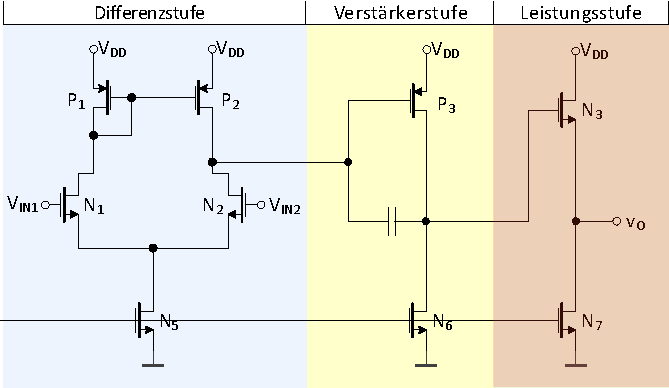
\includegraphics[width=0.8\columnwidth, align=t]{images/09_OpAmp_teile.pdf}
\end{center}

\vspace{-0.3cm}

\begin{minipage}[c]{0.58\columnwidth}
    \textrightarrow\ Jede Stufe hat ihre eigene Verstärkung $a_i$ \\
    \textrightarrow\ Die Gesamtverstärkung entspricht deren Produkt
\end{minipage}
\hfill
\begin{minipage}[b]{0.4\columnwidth}
    $$ a_{\rm OpAmp} = a_{\rm Diff} \cdot a_{\rm Gain} \cdot a_{\rm Leist} $$
\end{minipage}


\subsection{Differenzstufe -- Grosssignalanalyse\label{opamp:diff.stufe:grossignal}}

\subsubsection{Strong Inversion}

\begin{minipage}[t]{0.48\columnwidth}
    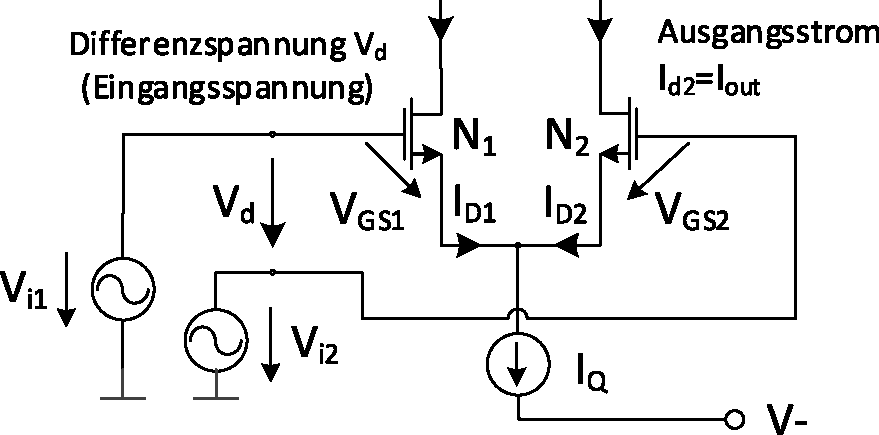
\includegraphics[width=\columnwidth, align=t]{images/09_differenzstufe_grosssignalanalyse.pdf}
\end{minipage}
\hfill
\begin{minipage}[t]{0.48\columnwidth}
    \begin{align*}
        \text{Sättigung:} \quad     I_\text{D}  &= \frac{\mu C_\text{ox}}{2} \frac{W}{L} (V_\text{GS} - V_\text{T})^2    \\
        \text{Konten:} \quad        I_\text{Q}  &= I_\text{D1} + I_\text{D2} 
    \end{align*}
\end{minipage}

\[
    \frac{I_\text{D}}{I_\text{Q}} = f(V_{\rm d}) = f(V_{i1} - V_{i2}) = \frac{1}{2} + \frac{1}{2} \sqrt{\frac{\left(\mu C_\text{ox} \frac{W}{L}\right) \cdot V_\text{d}^2}{I_\text{Q}} - \frac{\left(\mu C_\text{ox} \frac{W}{L}\right)^2 \cdot V_\text{d}^4}{4 I_\text{Q}}}
\]


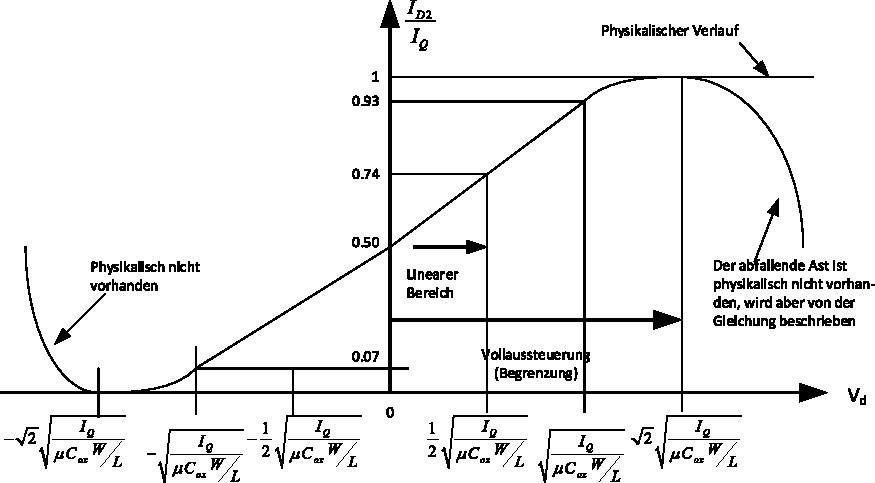
\includegraphics[width=\columnwidth, align=t]{images/09_differenzstufe_grosssignalanalyse_strong_inv.pdf}


\subsubsection{Weak Inversion}

\vspace{-0.2cm}

\[
    \text{Weak Inversion, Sättigung:} \qquad I_\text{D} = \frac{W}{L} I_\text{M}' e^\frac{V_\text{GS}-V_\text{M}}{n_\text{M} V_\text{temp}}
\]

\vspace{-0.2cm}

\[
    \frac{I_\text{D}}{I_\text{Q}} = f(V_{\rm d}) = f(V_{i1} - V_{i2}) = \frac{1}{2} \left(1 + \tanh \left( \frac{V_\text{d}}{2 n_\text{M} V_\text{temp}} \right) \right)
     \overset{V_d \text{ klein}}{\approx} \frac{1}{2} \left(1+\frac{V_\text{d}}{2 n_\text{M} V_\text{temp}}\right)
\]


\subsubsection{Conclusion Grosssignalanalyse}

Die \textbf{Verstärkung} ist im grossen und ganzen \textbf{unabhängig} von der Eingangsspannung und so \textbf{vom Arbeitspunkt}, der durch die Eingangsspannungen gegeben ist.

\smallskip

Der Ausgangsstrom hängt nur von der \textbf{Differenz der Eingangsspannungen} ab, was zu Linearität in einem grossen Bereich führt.


\subsection{Differenzstufe -- Kleinsignalanalyse}
\label{Differenzstufe -- Kleinsignalanalyse}

\subsubsection{Transkonduktanz $\bm{g_{\rm md}}$}


\begin{minipage}[t]{0.48\columnwidth}
    \paragraph{Widerstands- / Stromquellenlast}

    \[
        g_{\rm md} = \frac{i_{\rm out}}{v_{\rm d}} = - \frac{g_m}{2}
    \]
\end{minipage}
\hfill
\begin{minipage}[t]{0.48\columnwidth}
    \paragraph{Stromspiegellast}

    \[
        g_{\rm md} = \frac{i_{\rm out}}{v_{\rm d}} = - g_m
    \]
\end{minipage}


% TODO: [Flurin] Evtl. Schema und Ersatzschaltbild aus V10S11
%CHECK: [Simi] @Flurin There it is aber ich würde es weglassen... Habe im Bild weiter oben den 'Ort' eingefügt, wo die Last hin muss
% -> wenn du die Bilder verwenden willst, müsste man wahrscheinlich etwas umformatieren und herumschieben...

% \paragraph{Widerstandslast}

% \begin{minipage}[t]{0.45\columnwidth}
%     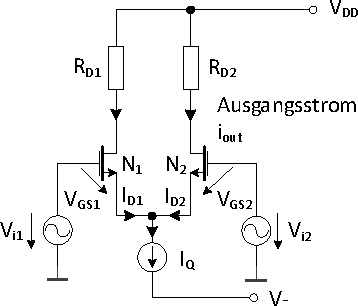
\includegraphics[width=\columnwidth, align=t]{images/09_differenzstufe_widerstandslast_schaltung.pdf}
% \end{minipage}
% \hfill
% \begin{minipage}[t]{0.45\columnwidth}
% 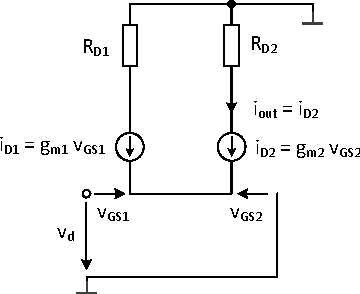
\includegraphics[width=\columnwidth, align=t]{images/09_differenzstufe_widerstandslast_kleinsignal.pdf}
% \end{minipage}


% \paragraph{Stromspiegellast}

% TODO: [Flurin] Evtl. Schema und Ersatzschaltbild aus V10S11
%CHECK: [Simi] @Flurin There it is aber ich würde es weglassen... Habe im Bild weiter oben den 'Ort' eingefügt, wo die Last hin muss
% -> wenn du die Bilder verwenden willst, müsste man wahrscheinlich etwas umformatieren und herumschieben...

% \begin{minipage}[t]{0.45\columnwidth}
%     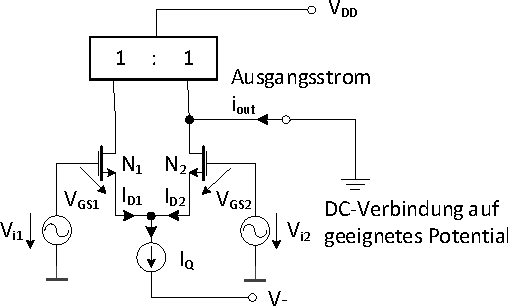
\includegraphics[width=\columnwidth, align=t]{images/09_differenzstufe_stromspiegellast_schaltung.pdf}
% \end{minipage}
% \hfill
% \begin{minipage}[t]{0.45\columnwidth}
%     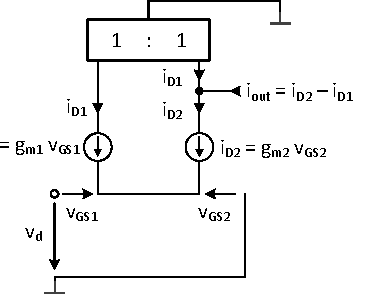
\includegraphics[width=\columnwidth, align=t]{images/09_differenzstufe_stromspiegellast_kleinsignal.pdf}
% \end{minipage}



\subsubsection{Verstärkung}

Generell berechnet sich die Verstärkung der Differenzstufe $a_{\rm Diff}$ als 

\[
    a_{\rm Diff} = \frac{v_{\rm out}}{v_{\rm in}} = g_{\rm md} \cdot r_{\rm Last\_tot}
\]

\begin{outline}
    \1 Abhängig von der Last muss $g_{\rm md}$ entsprechend eingesetzt werden
    \1 $r_{\rm Last\_tot}$ entspricht der gesamten Last am Ausgangsknoten
\end{outline}


\paragraph{Widerstandslast}

\begin{minipage}[t]{0.45\columnwidth}
    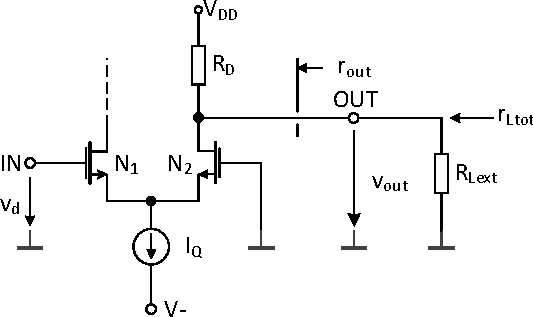
\includegraphics[width=\columnwidth, align=t]{images/09_differenzstufe_kleinsignal_verstaerkung_widerstand.pdf}
\end{minipage}
\hfill
\begin{minipage}[t]{0.5\columnwidth}
    \[
        r_{\rm Last\_tot} = \left( R_D \parallel r_{\rm DS} \parallel R_{\rm Lext} \right) \approx \left( R_D \parallel R_{\rm Lext} \right) 
    \]

    \[
        a_{\rm Diff} \approx - \frac{g_m (R_D \parallel R_{\rm Lext})}{2}
    \]
\end{minipage}



\paragraph{Stromspiegellast}

\begin{minipage}[t]{0.45\columnwidth}
    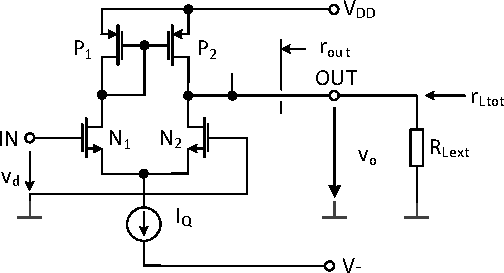
\includegraphics[width=\columnwidth, align=t]{images/09_differenzstufe_kleinsignal_verstaerkung_stromspiegel.pdf}
\end{minipage}
\hfill
\begin{minipage}[t]{0.5\columnwidth}
    \[
        r_{\rm Last\_tot} =  \left( r_{\rm DS\_N2} \parallel r_{\rm DS\_P2} \parallel R_{\rm Lext} \right)
    \]

    \vspace{-0.2cm}

    \[
        a_{\rm Diff} \approx - g_m \left(\frac{1}{g_{\rm o, N2}} \Biggm\Vert \frac{1}{g_{\rm o, N2}} \Biggm\Vert R_{\rm Lext}\right)
    \]
\end{minipage}


% \[
%     a \approx g_m \left(\frac{1}{g_{0, N2}} \Biggm\Vert \frac{1}{g_{0, N2}} \Biggm\Vert R_{L\text{, ext}}\right)
% \]


\paragraph{Stromquellenlast}    % NOTE: [Simi] Hat er nicht besprochen, daher verzichte ich hier auf das Schema

\vspace{-0.2cm}



\[
    r_{\rm Last\_tot} =  \left( r_{\rm QL} \parallel r_{\rm DS2} \parallel R_{\rm Lext} \right) \qquad \qquad
    a_{\rm Diff} \approx - \frac{ g_m \left( R_{\rm Lext} \parallel r_{\rm DS2} \parallel r_{\rm QL} \right) }{2}
\]



\subsubsection{Grenzwertbetrachtungen der Spannungsverstärkung}

Für folgende Grenzwertbetrachtungen der Spannungsverstärkung gilt: $R_{\rm Lext} = \infty$

\smallskip

\resizebox{\columnwidth}{!}{
    \renewcommand{\arraystretch}{1.5}
    \begin{tabular}{|l|l|l|}
        \hline
        \textbf{Betriebsbereich}    & \textbf{Grenzwert der Spannungsverstärkung}                                                                                                       & \textbf{Grössere Verstärkung bei}                                         \\
        \hline
        Strong Inversion            & $\displaystyle \abs{a_{\text{max}}} = 2 V_e \sqrt{\frac{\mu C_\text{ox} \frac{W}{L}}{I_Q}} \approx 2 a_E \sqrt{\frac{\mu C_\text{ox} L W}{I_Q}}$  & Ruhestrom $\downarrow$, Fläche $\uparrow$, (Early-Spannung $\uparrow$)    \\
        \hline
        Weak Inversion              & $\abs{a_{\text{max}}} = \frac{V_E}{n_M V_\text{temp}} \approx \frac{a_E L}{n_M V_\text{temp}}$                                                    & (Early-Spannung $\uparrow$)                                               \\
        \hline
    \end{tabular}
    \renewcommand{\arraystretch}{1}
}

\medskip

Diese Formeln sollten \textbf{nicht zur Verstärkungsberechnung verwendet werden} -- sie dienen lediglich zur Veranschaulichung der Bezüge verschiedener Parameter.
% TODO: [Flurin] Evtl mehr Formeln / Bedingungen aus V10S14?
% [Simi] @Flurin: Ich würde nicht... Wir dürfen damit ja sowieso nicht rechnen....




\subsection{Verstärkerstufe}
Für die Verstärkerstufe wird in der Regel eine Source-Schaltung mit Stromquellenlast eingesetzt.
Diese hat eine Verstärkung von

\vspace{-0.2cm}
\[
    a_{\rm Gain} = - g_m (r_{DS1} \parallel r_Q)
\]


\subsection{Leistungsstufe}
Als Leistungsstufe wird für Closed-Loop Anwendungen meist eine Drain-Stufe mit Stromquellenlast verwendet.
Diese hat eine Verstärkung von
\vspace{-0.2cm}

\[
    a_{\rm Leist} \approx 1
\]

Die Verstärkung der Leistungsstufe ist dabei $\leq 1$ um Instabilität zu vermeiden. \\
In Open-Loop Anwendungen darf die Leistungsstufe auch Verstärkungen $>1$ aufweisen.


\subsection{Kenngrössen}

\subsubsection{Gain-Bandwidth-Product GBW}
\vspace{-0.2cm}

\[
    \text{GBW} = \abs{a} \cdot  f_d \quad (= \text{GBP}) 
    \qquad \qquad \qquad
    \text{BW} = \frac{\text{GBW}}{a} \quad \Leftrightarrow\ \quad a = \frac{\text{GBW}}{\text{BW}}  % CHECK [Simi] @Flurin \abs{a} statt a ?
\]

% \begin{tabular}{ll | ll | ll}
%     $f_d$   & Frequenz des dominanten (ersten) Pols     & $a$   & Verstärkung   & $B$   & Bandbreite           
% \end{tabular}

\begin{tabular}{l | l | l}
    $f_d:$ Frequenz des dominanten (ersten) Pols    & $a:$ Verstärkung   & BW: Bandbreite           
\end{tabular}


% $f_d$: Frequenz des dominanten (ersten) Pols.
% Es gilt schliesslich für alle Verstärkungen $a$
% \[
%     B = \frac{GBW}{a} \quad \text{bzw.} \quad a = \frac{GBW}{B}
% \]



\paragraph{Beispiel Differenzstufe}
\[
    a = -g_m R_{\rm out} \quad \text{und} \quad f_d = \frac{1}{2 \pi R_{\rm out} C_L}
\]
\begin{center}
    \textdownarrow
\end{center}
\[
    \text{GBW} = \abs{a} \cdot f_d = \abs{-g_m R_{\rm out}} \cdot \frac{1}{2 \pi R_{\rm out} C_L} = \frac{g_m}{2 \pi C_L}
\]

\subsubsection{Slew-Rate}
Die Slew-Rate beschreibt die maximale Ausgangsspannungsänderung pro Zeiteinheit:

\[
    \text{SR} = \text{SR}_r = \abs{\text{SR}_f} = \frac{\diff v_o}{\diff t} \Bigg|_{\rm max} = \frac{I_Q}{C_L}
\]
\paragraph{Aussteuerung als Funktion der Eingangsfrequenz}
Die Aussteuerung $\Delta V$ des Ausgangs bei einem Rechteck am Eingang berechnet isch als % CHECK: [Flurin] nur für Rechteck oder für andere Signale auch?!
\[
    \Delta V = f(\text{SR, \, f}) = \text{SR} \cdot \Delta t = \frac{\text{SR}}{2 f} = \frac{I_Q}{C_L \cdot 2 f}
\]


\paragraph{Bestimmung der Slew Rate bei mehrstufigen Verstärkern}

\begin{minipage}[t]{0.46\columnwidth}
    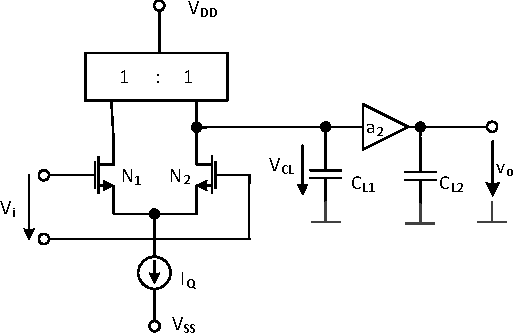
\includegraphics[width=\columnwidth, align=t]{images/09_slew_rate.pdf}
\end{minipage}
\hfill
\begin{minipage}[t]{0.5\columnwidth}
    Eine Stufe limitiert die Slew Rate der gesamten Schaltung. 
    Um die limitierende (dominante) Stufe zu bestimmen, wird folgendermassen vorgegangen:

    \smallskip

    \begin{enumerate}
        \item SR jeder Stufe einzeln bestimmen.
        \item Berechneten Wert auf den Ausgang normieren \textrightarrow\ $\text{SR}_{\rm out} = \text{SR}_i \cdot a$
        \item Kleinste normierte SR wählen \\
            \textrightarrow\ entspricht limitierender Stufe
    \end{enumerate}
\end{minipage}


\paragraph{Designregeln}
\begin{itemize}
    \item Hohe Slew Rate: $I_Q$ \textuparrow, $C_L$ \textdownarrow, Stromverbrauch \textuparrow%
    \item Frequenzkompensation ($C_C$) reduziert die Slew-Rate
\end{itemize}


\subsubsection{Eingangsspannungsbereich}
\paragraph{Gleichtakt / Common-Mode}

\begin{minipage}[t]{0.36\columnwidth}
    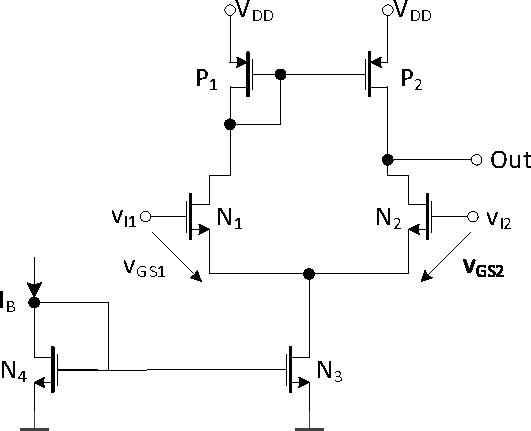
\includegraphics[width=\columnwidth, align=t]{images/09_common_mode_range.pdf}
\end{minipage}
\hfill
\begin{minipage}[t]{0.58\columnwidth}
    \[
        V_{\rm inCM} = \frac{V_{\rm in1} + V_{\rm in2}}{2}
    \]
    
    \vspace{-0.5cm}

    \begin{align*}
        V_{\rm inCM, min}   &= V_{\rm SS} + V_{\rm DS,satN3} + V_{\rm GS,N1/N2} \\
        V_{\rm inCM, max}   &= V_{\rm DD} - V_{\rm GS,P1} - V_{\rm DS,sat,N1} + V_{\rm GS,N1} \\
                            &= V_{\rm DD} - V_{\rm GS,P1} + V_{\rm th,N} 
    \end{align*}
\end{minipage}

\smallskip

Bei Unterschreitung von $V_{\rm inCM, min}$ fällt der Transistor $N_3$ durch Reduktion des Stroms aus dem Stromquellenbereich in den Widerstandsbereich. Dies reduziert das $g_m$.

Bei Überschreitung von $V_{\rm inCM, max}$ fallen die Transistoren $P_1$ und $P_2$ aus der Sättigung, was den Stromspiegel unwirksam macht. Auch dies reduziert das $g_m$.


\paragraph{Gegentakt / Differential-Mode}
\[
    V_{\rm inDM} = V_{\rm in1} - V_{\rm in2}
\]
Der Gegentakt-Eingangsspannungsbereich kann der Grossignalanalyse in~\ref{opamp:diff.stufe:grossignal} entnommen werden.


\subsubsection{Common-Mode-Rejection}
\paragraph{Berechnung}

Durch Symmetrie kann zur Berechnung der Common-Mode-Verstärkung die Stromquelle 'halbiert' werden.
%TODO: [Flurin] Schema aus V11S14, ich glaube erklärende Schemen zu CM und DM sind nicht nötig.
%CHECK: [Simi] @Flruin: Habe ich dich jetzt richtig verstanden mit diesem Schema...?

\begin{minipage}[t]{0.48\columnwidth}
    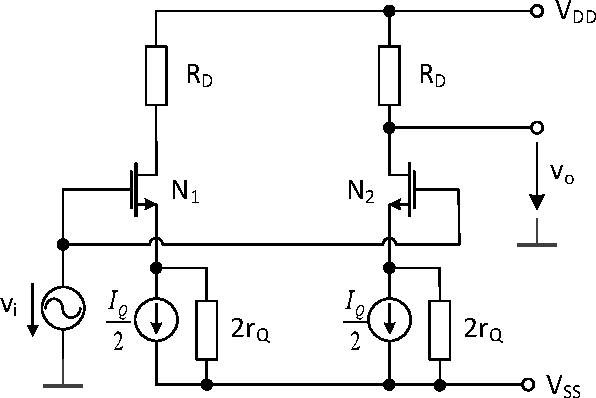
\includegraphics[width=\columnwidth, align=t]{images/09_common_mode_rejection.pdf}
\end{minipage}
\hfill
\begin{minipage}[t]{0.48\columnwidth}
    Folglich kann zur Berechnung die Formel der Source-Schaltung verwenden:
    \[
        a_{\rm CM} \approx - \frac{R_D}{2 r_Q}
    \]

    Die Differential-Mode-Verstärkung kann wie gehabt berechnet werden:
    \[
        a_{\rm DM} \approx -\frac{g_m}{2} R_D
\]
\end{minipage}



\paragraph{Minimierung der Common-Mode-Verstärkung}
Die Common-Mode-Verstärkung kann durch Wahl einer guten Stromquelle ($r_Q >> 2 \cdot R_D$) minimiert werden.

\paragraph{Common-Mode-Rejection-Ratio}

\vspace{-0.2cm}

\[
    \text{CMRR} = \abs{\frac{a_{\rm DM}}{a_{\rm CM}}} = \abs{\frac{-\frac{g_m}{2} R_D}{- \frac{R_D}{2 r_Q}}} = g_m \cdot r_Q = \frac{g_m}{g_{\rm oQ}}
\]
% Mit
% \[
%     a_{CM} \approx \frac{R_D}{2 r_Q} \quad \text{und} \quad
%     a_{DM} \approx -\frac{g_m}{2} R_D
% \]
% folgt
% \[
%     CMRR = \abs{\frac{-\frac{g_m}{2} R_D}{\frac{R_D}{2 r_Q}}} = g_m \cdot r_Q
% \]

\subsubsection{Speisungsspannungsunterdrückung}

% \paragraph{Intuitiv}

\begin{minipage}[c]{0.68\columnwidth}
    \begin{itemize}
        \item Die Rejection von Störungen auf dem Bezugspotential von Verstärkern werden recht direkt auf den Ausgang übertragen.
        \item Speisungen, die über eine Stromquelle mit der Verstärkerschaltung verbunden sind, werden mit dem Innenwiderstand dieser Quellen gedämpft.
    \end{itemize}
\end{minipage}
\hfill
\begin{minipage}[c]{0.3\columnwidth}
    \[
        \text{PSRR}_+ = \abs{\frac{a_{\rm DM}}{a_{\rm PS+}}}
    \]
    \[
        \text{PSRR}_- = \abs{\frac{a_{\rm DM}}{a_{\rm PS-}}}
    \]
\end{minipage}


\subsubsection{Offset}

\paragraph{Random Offset}
Entsteht durch \textbf{Prozessvariationen}.
\begin{itemize}
    \item Das Matching der Eingangstransistoren kann durch Common-Centroid-Layout optimiert werden
    \item $V_{\rm GS} - V_T$ nicht minimal wählen
    \item Grosses $W/L$ für Eingangstransistoren
\end{itemize}


\paragraph{Systematic Offset}
Entsteht durch \textbf{schaltungstechnische Asymmetrien} und können durch Befolgen folgender Design Rules eliminiert werden.

\vspace{-0.2cm}

\begin{center}
    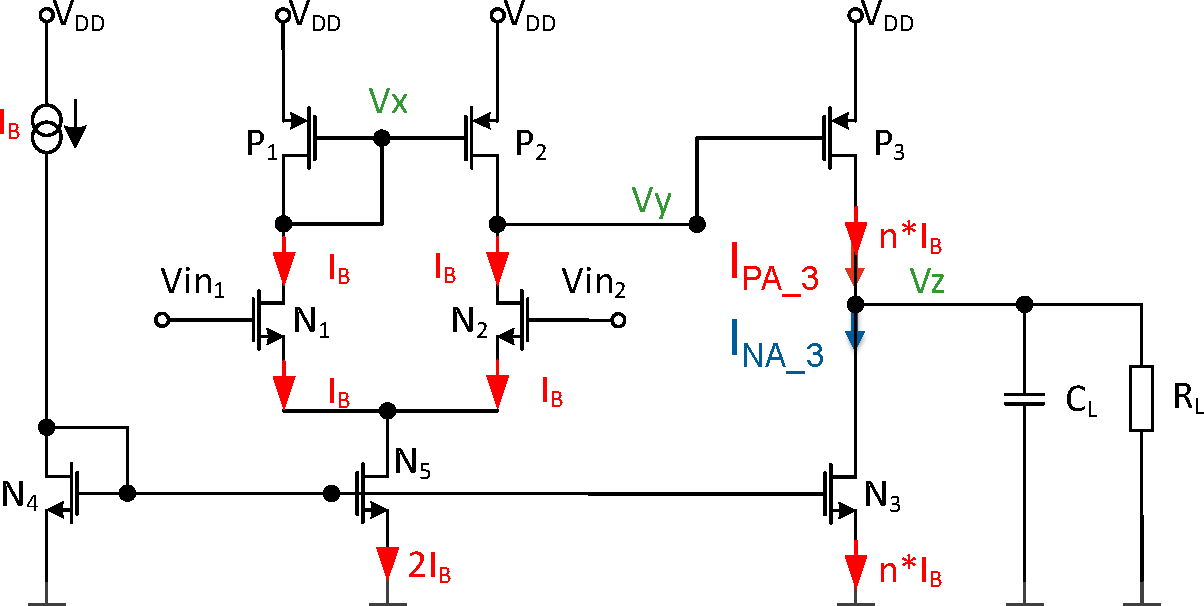
\includegraphics[width=0.8\columnwidth, align=t]{images/09_offset.pdf}
\end{center}

\begin{outline}
    \1 Identisches $L$ der Stromspiegeltransistoren $N_3 - N_5$ sowie $P_1$ und $P_2$ ($\lambda$ identisch)
    \1 Diff. Stufe symmetrisch, damit Ströme identisch ($V_{in1} = V_{in2}$)
        \2 $N_1$ und $N_2$ sowie $P_1$ und $P_2$ identisch
        \2 $V_x$ = $V_y$ \textrightarrow\ gleiches $V_{\rm GS}$ und $V_{\rm DS}$ für $N_1$ und $N_2$ resp. $P_1$ und $P_2$
    \1 Ausgangsstufe $P_3$ spiegelt $I_{\rm P1,2}$ ideal: $I_{\rm P3} = I_{\rm N3} = n \cdot I_B$
        \2 gleiches $V_{\rm GS}$ ($V_x = V_y$) und $V_{\rm DS}$ ($V_y = V_z = V_{\rm out_o}$) für $P_2$ und $P_3$
        \2 \textbf{gleiche Stromdichte:} $\bm{I_{\rm P1} / (W/L)_{\rm P1} = I_{\rm P2} / (W/L)_{\rm P2} = I_{\rm P3} / (W/L)_{\rm P3} }$
\end{outline}

